\documentclass[tikz,border=8pt]{standalone}
% Shared look for every TikZ diagram. Load with \input{../../tools/tikz-style.tex}
\usepackage[T1]{fontenc}
\usepackage{lmodern}
\renewcommand{\sfdefault}{lmr}  % diagrams use the same serif as the text
\usetikzlibrary{arrows.meta, positioning, shapes.geometric, calc, fit, backgrounds}
\definecolor{cblue}{HTML}{4C78A8}
\definecolor{corange}{HTML}{F58518}
\definecolor{cgreen}{HTML}{54A24B}
\definecolor{cred}{HTML}{E45756}
\definecolor{cpurple}{HTML}{B279A2}
\definecolor{cgrey}{HTML}{6B6B6B}
\tikzset{
  every picture/.style={font=\sffamily, line width=1.2pt},
  box/.style={draw=#1, fill=#1!12, rounded corners=4pt, align=center, inner sep=7pt, minimum height=1.1cm},
  box/.default=cgrey,
  arrow/.style={-{Stealth[length=3mm]}, draw=cgrey, line width=1.4pt},
  title/.style={font=\sffamily\bfseries\Large},
  note/.style={font=\sffamily\small, text=cgrey, align=center},
}
\AtBeginDocument{\hyphenpenalty=10000 \exhyphenpenalty=10000}

\begin{document}
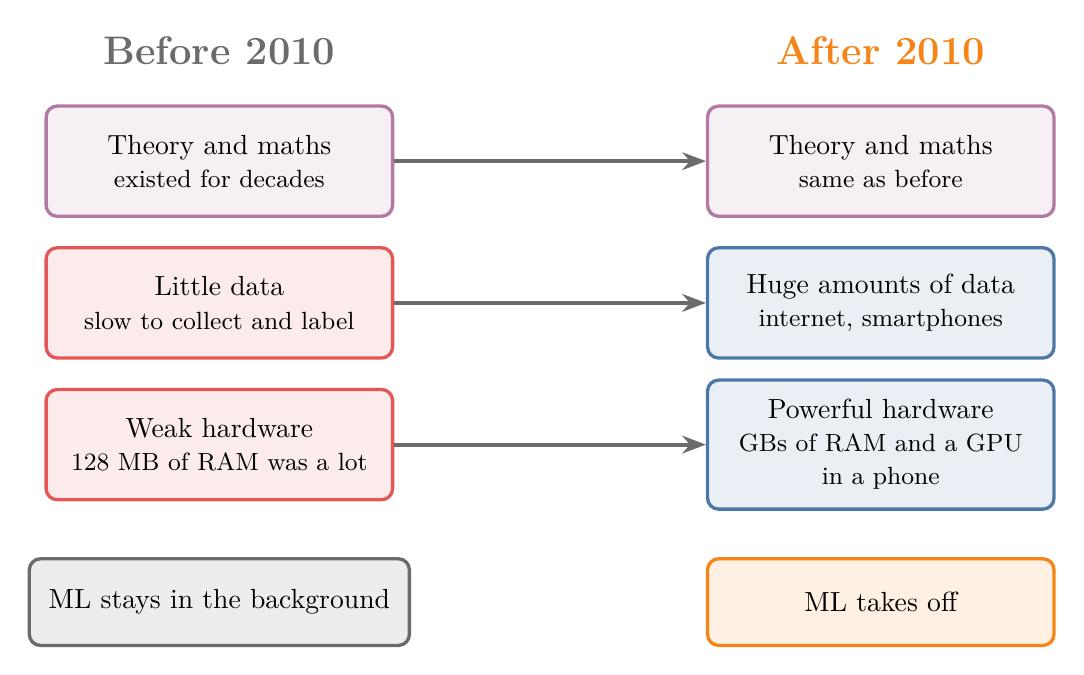
\begin{tikzpicture}
  \node[title, cgrey] at (0,3.2) {Before 2010};
  \node[title, corange] at (8.4,3.2) {After 2010};
  % rows
  \node[box=cpurple, minimum width=4.4cm, minimum height=1.4cm] (t1) at (0,1.8) {Theory and maths\\{\small existed for decades}};
  \node[box=cpurple, minimum width=4.4cm, minimum height=1.4cm] (t2) at (8.4,1.8) {Theory and maths\\{\small same as before}};
  \node[box=cred, minimum width=4.4cm, minimum height=1.4cm] (d1) at (0,0) {Little data\\{\small slow to collect and label}};
  \node[box=cblue, minimum width=4.4cm, minimum height=1.4cm] (d2) at (8.4,0) {Huge amounts of data\\{\small internet, smartphones}};
  \node[box=cred, minimum width=4.4cm, minimum height=1.4cm] (h1) at (0,-1.8) {Weak hardware\\{\small 128 MB of RAM was a lot}};
  \node[box=cblue, minimum width=4.4cm, minimum height=1.4cm] (h2) at (8.4,-1.8) {Powerful hardware\\{\small GBs of RAM and a GPU}\\{\small in a phone}};
  \draw[arrow] (t1) -- (t2); \draw[arrow] (d1) -- (d2); \draw[arrow] (h1) -- (h2);
  \node[box=cgrey, minimum width=4.4cm] (r1) at (0,-3.8) {ML stays in the background};
  \node[box=corange, minimum width=4.4cm] (r2) at (8.4,-3.8) {ML takes off};
\end{tikzpicture}
\end{document}
